\chapter{Perancangan}
Bab ini akan membahas mengenai perancangan aplikasi. Perancangan aplikasi akan meliputi tampilan antarmuka, diagram kelas lengkap beserta dengan deskripsi dan fungsinya.

\section{Perancangan Antarmuka}
\label{perancangan_antarmuka}

Agar pengguna dapat menggunakan perangkat lunak ini dengan nyaman, maka dibutuhkan antarmuka. Rancangan antarmuka yang dibuat terdiri dari satu \textit{frame} dan di dalamnya terdapat beberapa \textit{tab}, yaitu \textit{tab embed}, \textit{tab extract}, \textit{tab} tambah \textit{cover}, \textit{tab} tambah sinonim, dan \textit{tab} petunjuk seperti yang dapat dilihat pada Gambar \ref{fig:0-tab}(1).

\begin{figure}[H]
	\centering
	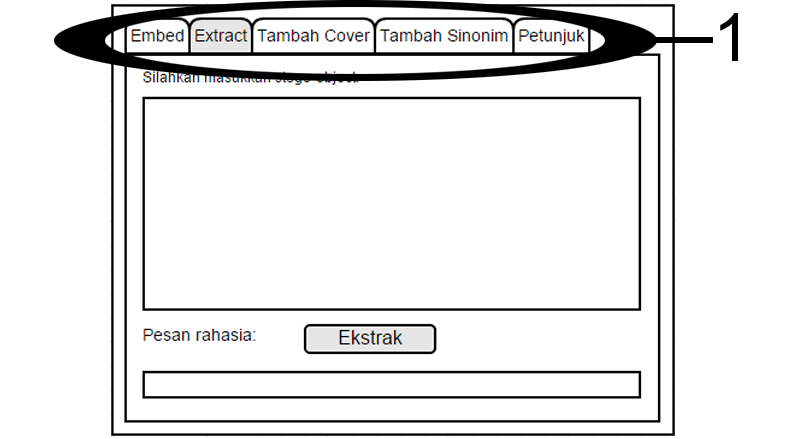
\includegraphics[scale=1.8]{Gambar/tab}
	\caption{Tampilan \textit{tab}} 
	\label{fig:0-tab}
\end{figure}

\subsection{\textit{Tab Embed}}

\begin{figure}[H]
	\centering
	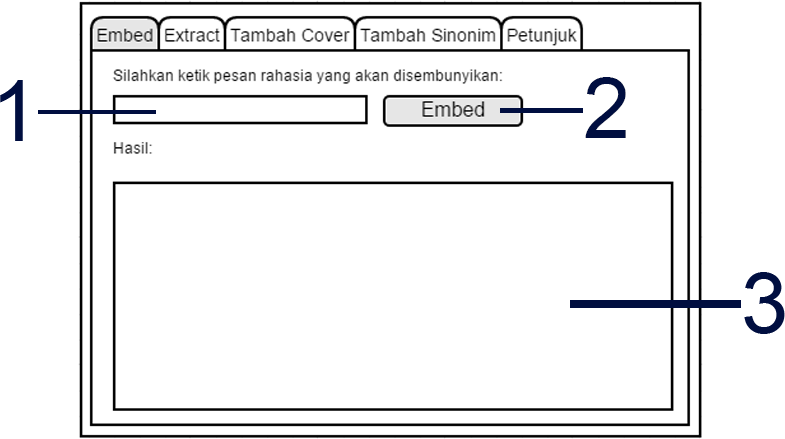
\includegraphics[scale=1.8]{Gambar/tab-embed}
	\caption{Tampilan \textit{tab Embed}} 
	\label{fig:1-tab-embed}
\end{figure}

Pada \textit{tab Embed} (dapat dilihat pada Gambar \ref{fig:1-tab-embed}) terdapat beberapa elemen sebagai berikut.

\begin{enumerate}
	\item \textbf{\textit{Text box secret message}}, pengguna dapat mengetikkan pesan rahasia yang akan disembunyikan pada bagian ini.
	\item \textbf{Tombol \textit{Embed}}, pengguna dapat menekan tombol ini untuk melakukan proses \textit{embedding}.
	\item \textbf{\textit{Text area stego-object}}, hasil proses \textit{embedding} yang merupakan \textit{stego-object} akan muncul pada bagian ini.
\end{enumerate}

\subsection{\textit{Tab Extract}}

\begin{figure}[H]
	\centering
	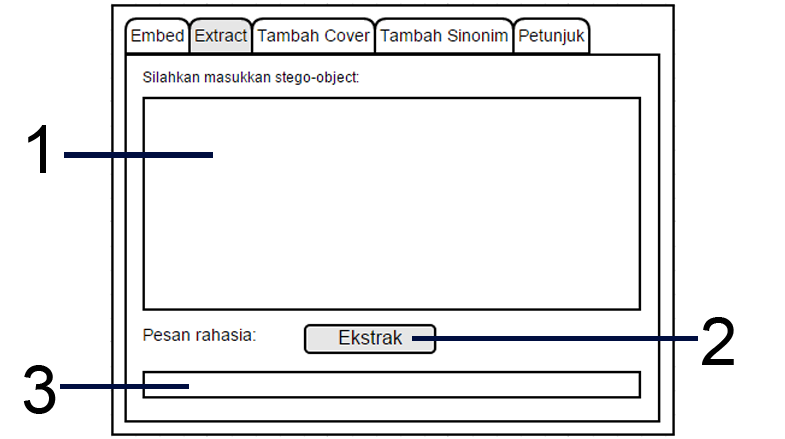
\includegraphics[scale=1.8]{Gambar/tab-extract}
	\caption{Tampilan \textit{tab Extract}} 
	\label{fig:2-tab-extract}
\end{figure}

Pada \textit{tab Extract} (dapat dilihat pada Gambar \ref{fig:2-tab-extract}) terdapat beberapa elemen sebagai berikut.

\begin{enumerate}
	\item \textbf{\textit{Text area stego-object}}, pengguna dapat memasukkan \textit{stego-object} yang diterima pada bagian ini.
	\item \textbf{Tombol Ekstrak}, pengguna dapat menekan tombol ini untuk melakukan proses \textit{extracting}.
	\item \textbf{\textit{Text box secret message}}, hasil \textit{extracting} akan ditampilkan pada bagian ini.
\end{enumerate} 

\subsection{\textit{Tab} Tambah \textit{Cover}}

\begin{figure}[H]
	\centering
	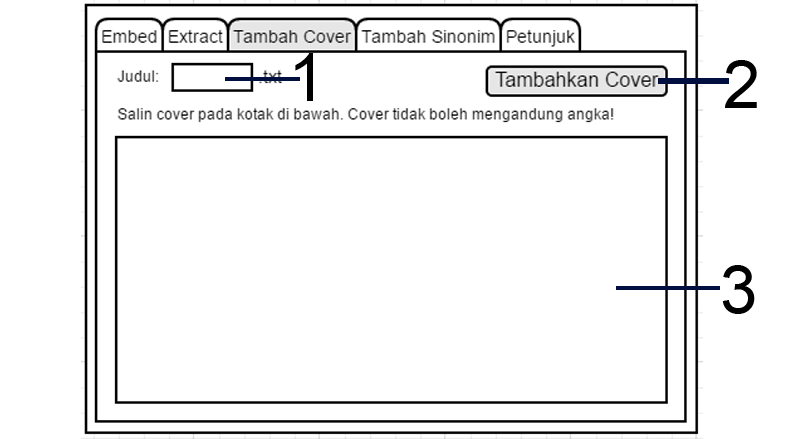
\includegraphics[scale=1.8]{Gambar/tab-tambah-cover}
	\caption{Tampilan \textit{tab} Tambah \textit{Cover}} 
	\label{fig:3-tab-tambah-cover}
\end{figure}

Pada \textit{tab} Tambah \textit{Cover} (dapat dilihat pada Gambar \ref{fig:3-tab-tambah-cover}) terdapat beberapa elemen sebagai berikut.

\begin{enumerate}
	\item \textbf{\textit{Text box} judul}, pengguna dapat mengetikkan judul dari \textit{stego-cover} yang akan ditambahkan pada bagian ini.
	\item \textbf{Tombol Tambah \textit{Cover}}, pengguna dapat menekan tombol ini untuk menambahkan \textit{stego-cover} yang telah disalin pada no 3.
	\item \textbf{\textit{Text area stego-cover}}, pengguna dapat menyalin \textit{stego-cover} yang memenuhi persyaratan di bagian ini.
	\item \textbf{Label peringatan}, peringatan akan muncul jika pengguna belum memasukkan judul \textit{file}, judul yang diketik telah terdaftar, atau saat \textit{stego-cover} berhasil ditambahkan.
\end{enumerate} 

\subsection{\textit{Tab} Tambah Sinonim}

\begin{figure}[H]
	\centering
	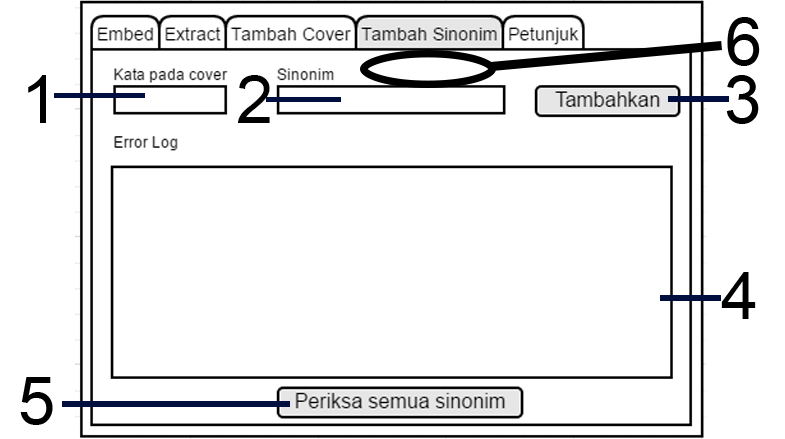
\includegraphics[scale=1.8]{Gambar/tab-tambah-sinonim}
	\caption{Tampilan \textit{tab} Tambah Sinonim} 
	\label{fig:4-tab-tambah-sinonim}
\end{figure}

Pada \textit{tab} Tambah Sinonim (dapat dilihat pada Gambar \ref{fig:4-tab-tambah-sinonim}) terdapat beberapa elemen sebagai berikut.

\begin{enumerate}
	\item \textbf{\textit{Text box} kata pada \textit{cover}}, kata pada \textit{cover} berarti kata yang ada pada \textit{stego-cover}, pengguna dapat mengetikkannya pada bagian ini.
	\item \textbf{\textit{Text box} sinonim}, pengguna dapat mengetik sinonimnya pada bagian ini.
	\item \textbf{Tombol Tambahkan}, pengguna dapat menekan tombol ini untuk memasukkan pasangan kata dan sinonim yang baru ke \textit{file} kamus.
	\item \textbf{\textit{Text Area} Error Log}, akan menampilkan daftar kata yang belum memiliki sinonim jika pengguna menekan tombol Periksa semua sinonim.
	\item \textbf{Tombol Periksa semua sinonim}, akan memeriksa semua kata dari tiap \textit{stego-cover} yang terdaftar dan menampilkan daftar kata yang belum memiliki sinonim.
	\item \textbf{Label peringatan}, akan memberikan keterangan jika sinonim gagal atau berhasil ditambahkan.
\end{enumerate} 

\subsection{\textit{Tab} Petunjuk}

\begin{figure}[H]
	\centering
	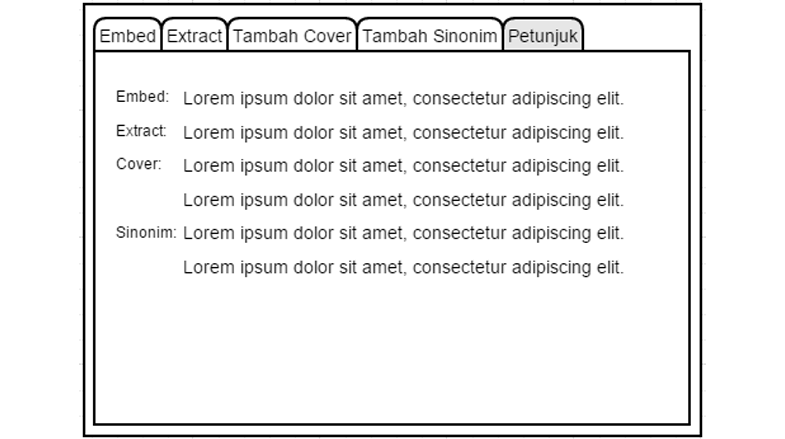
\includegraphics[scale=1.8]{Gambar/tab-petunjuk}
	\caption{Tampilan \textit{tab} Petunjuk} 
	\label{fig:5-tab-petunjuk}
\end{figure}

\textit{Tab} Petunjuk (dapat dilihat pada Gambar \ref{fig:5-tab-petunjuk}) sebenarnya hanya dibuat untuk membantu pengguna yang baru pertama kali memakai perangkat lunak ini. Pada \textit{tab} ini berisi petunjuk-petunjuk yang dapat membantu pengguna untuk mengoperasikan perangkat lunak ini.

\section{Diagram Kelas Lengkap}

Diagram kelas sebelumnya yang dapat dilihat pada Gambar \ref{fig:3_classdiagram} mengalami beberapa perubahan dan penambahan kelas. Diagram kelas lengkap dapat dilihat pada Gambar \ref{fig:6-class-diagram-lengkap}.

Deskripsi setiap kelas beserta dengan atribut dan fungsinya akan dijelaskan sebagai berikut.

\begin{enumerate}
	\item Kelas PemotongKata\\
	Kelas ini merupakan kelas yang merepresentasikan pemotong kata. Fungsi-fungsi yang ada pada kelas ini adalah:
	\begin{itemize}
		\item \textbf{public String getPattern(String input)} \\
		Berfungsi untuk mendapatkan pola suku kata (KV, K, V, dst.).\\
		\textbf{Parameter:}
		\begin{itemize}
			\item \textbf{input} Teks yang akan didapatkan pola suku katanya.
		\end{itemize}
		
		\item \textbf{public ArrayList generateLevel1(String text)} \\
		Berfungsi untuk melakukan DFSA tahap 1.\\
		\textbf{Parameter:}
		\begin{itemize}
			\item \textbf{text} Teks yang akan didapatkan suku katanya.
		\end{itemize}
		
		\item \textbf{public ArrayList generateLevel2(ArrayList lv1)}\\
		Berfungsi untuk melakukan DFSA tahap 2.\\
		\textbf{Parameter:}
		\begin{itemize}
			\item \textbf{lv1} Merupakan kembalian dari fungsi generateLevel1().
		\end{itemize}
		
		\item \textbf{public ArrayList generateLevel3(ArrayList lv2)}\\
		Berfungsi untuk melakukan DFSA tahap 3.\\
		\textbf{Parameter:}
		\begin{itemize}
			\item \textbf{lv2} Merupakan kembalian dari fungsi generateLevel2().
		\end{itemize}
		
		\item \textbf{public int getJumlahSukuKata(String in)}\\
		Berfungsi untuk menghitung banyaknya suku kata.\\
		\textbf{Parameter:}
		\begin{itemize}
			\item \textbf{in} Merupakan teks yang akan dicari banyak suku katanya.
		\end{itemize}
	\end{itemize}
	
	\begin{figure}[H]
		\centering
		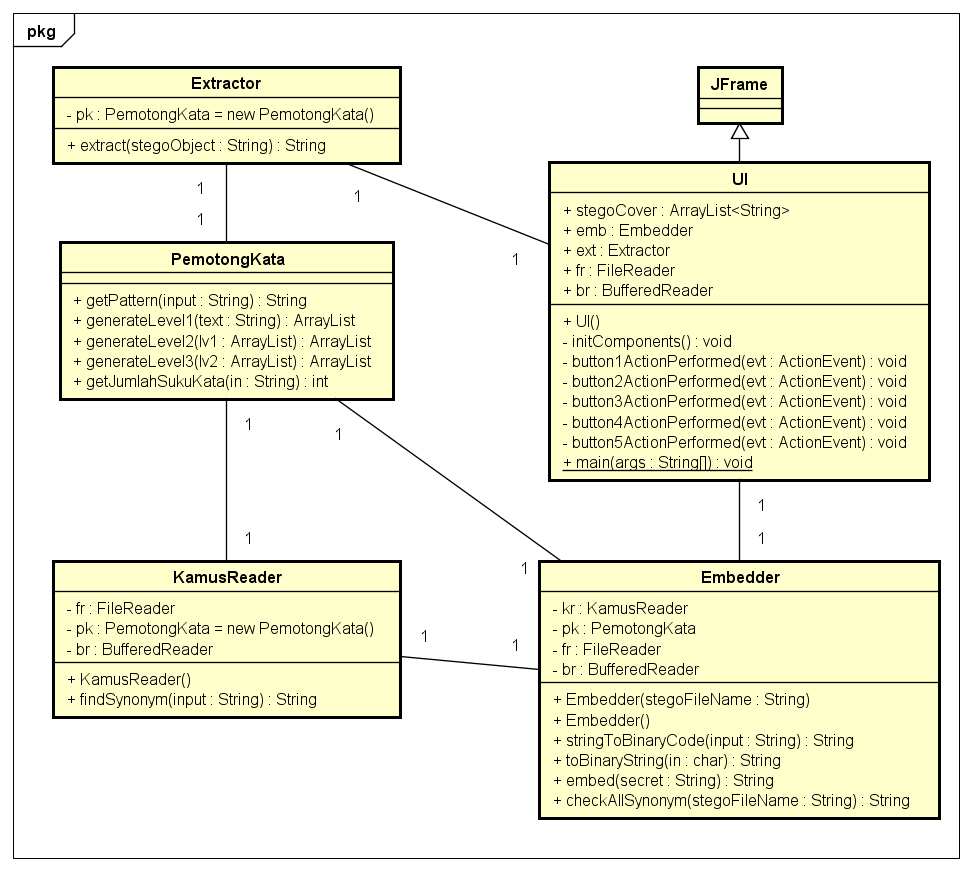
\includegraphics[scale=0.6]{Gambar/class-diagram-lengkap}
		\caption{Diagram kelas lengkap} 
		\label{fig:6-class-diagram-lengkap}
	\end{figure}	
	
	\item Kelas KamusReader\\
	Kelas ini berfungsi untuk membaca \textit{file} kamus dengan tujuan mencari sinonim. Atribut yang ada pada kelas KamusReader adalah:
	\begin{itemize}
		\item \textbf{FileReader fr:} Objek FileReader yang berfungsi untuk membuka suatu \textit{file}.
		\item \textbf{BufferedReader br:} Objek BufferedReader yang berfungsi untuk membaca isi dari \textit{file} yang dibuka FileReader.
		\item \textbf{PemotongKata pk:} Objek PemotongKata yang akan berfungsi untuk memotong kata.
	\end{itemize}
	
	Fungsi-fungsi yang dimiliki kelas ini adalah:
	
	\begin{itemize}
		\item \textbf{KamusReader()}\\
		Merupakan \textit{constructor} dari kelas KamusReader yang akan menginisialisasi atribut-atributnya.
		\item \textbf{String findSynonym(String input)}\\
		Berfungsi untuk mencari sinonim dari parameter.\\
		\textbf{Parameter:}
		\begin{itemize}
			\item \textbf{input} Kata yang akan dicari sinonimnya.
		\end{itemize}
	\end{itemize}
	
	\item Kelas Embedder\\
	Kelas ini berfungsi untuk menangani seluruh kegiatan \textit{embedding} pesan ke dalam \textit{stego-cover}. Atribut yang ada pada kelas Embedder adalah:
	\begin{itemize}
		\item \textbf{KamusReader kr:} Objek KamusReader berfungsi untuk membaca \textit{file} kamus.
		\item \textbf{PemotongKata pk:} Objek PemotongKata berfungsi untuk memotong kata.
		\item \textbf{FileReader fr:} Objek FileReader yang berfungsi untuk membuka suatu \textit{file}.
		\item \textbf{BufferedReader br:} Objek BufferedReader yang berfungsi untuk membaca isi dari \textit{file} yang dibuka FileReader.
	\end{itemize}
	
	Fungsi-fungsi yang dimiliki kelas ini adalah:
	
	\begin{itemize}
		\item \textbf{Embedder(String stegoFileName)}\\
		Merupakan \textit{constructor} dari kelas Embedder dengan parameter nama \textit{stego-cover} yang akan langsung dibuka oleh FileReader.\\
		\textbf{Parameter:}
		\begin{itemize}
			\item \textbf{stegoFileName} Nama \textit{file stego-cover} yang akan dibuka oleh FileReader.
		\end{itemize}
		
		\item \textbf{Embedder()}\\
		Merupakan \textit{constructor} tanpa parameter dari kelas Embedder yang akan menginisialisasi FileReader dan BufferedReader.
		
		\item \textbf{String stringToBinaryCode(String input)}\\
		Berfungsi untuk mengubah setiap karakter dalam string menjadi biner.\\
		\textbf{Parameter:}
		\begin{itemize}
			\item \textbf{input} String yang akan diubah menjadi biner.
		\end{itemize}
		
		\item \textbf{String toBinaryString(char in)}\\
		Berfungsi untuk mendapatkan kode ASCII dari karakter.\\
		\textbf{Parameter:}
		\begin{itemize}
			\item \textbf{in} Karakter yang akan didapatkan kode ASCII-nya.
		\end{itemize}
		
		\item \textbf{String embed(String secret)}\\
		Berfungsi untuk melakukan proses \textit{embedding}.\\
		\textbf{Parameter:}
		\begin{itemize}
			\item \textbf{secret} Pesan rahasia yang akan disembunyikan.
		\end{itemize}
		
		\item \textbf{String checkAllSynonym(String stegoFileName)}\\
		Berfungsi untuk cek kata mana saja (yang ada pada \textit{stego-cover}) yang sinonimnya belum terdaftar pada kamus sinonim.\\
		\textbf{Parameter:}
		\begin{itemize}
			\item \textbf{stegoFileName} Nama \textit{file stego-cover} yang akan dicek.
		\end{itemize}
	\end{itemize}
	
	\item Kelas Extractor\\
	Kelas ini berfungsi untuk menangani seluruh kegiatan \textit{extracting} pesan dari \textit{stego-object}. Atribut yang ada pada kelas Extractor adalah:
	\begin{itemize}
		\item \textbf{PemotongKata pk:} Objek PemotongKata berfungsi untuk memotong kata.
	\end{itemize}
	
	Fungsi-fungsi yang dimiliki kelas ini adalah:
	
	\begin{itemize}	
	
		\item \textbf{String extract(String stegoObject)}\\
		Berfungsi untuk melakukan proses \textit{extracting}\\
		\textbf{Parameter:}
		\begin{itemize}
			\item \textbf{stegoObject} \textit{Stego-object} yang akan diekstrak.
		\end{itemize}
				
	\end{itemize}
	
	
	
	\item Kelas UI
	Kelas ini merupakan antarmauka yang berhubungan langsung dengan pengguna. Kelas ini merupakan turunan dari kelas JFrame. Atribut yang ada pada kelas UI adalah:
	\begin{itemize}
		\item \textbf{ArrayList<String> stegoCover:} Objek stegoCover menyimpan judul-judul \textit{stego-cover} yang ada.
		\item \textbf{Embedder emb:} Objek \textit{Embedder} berfungsi untuk melakukan operasi \textit{embedding}.
		\item \textbf{Extractor ext:} Objek \textit{Extractor} berfungsi untuk melakukan operasi \textit{extracting}.
		\item \textbf{FileReader fr:} Objek FileReader yang berfungsi untuk membuka suatu \textit{file}.
		\item \textbf{BufferedReader br:} Objek BufferedReader yang berfungsi untuk membaca isi dari \textit{file} yang dibuka FileReader.
	\end{itemize}
	
		Fungsi-fungsi yang dimiliki kelas ini adalah:
		
	\begin{itemize}
		\item \textbf{UI()}\\
		Berfungsi sebagai \textit{constructor} kelas ini.\\	
		
		\item \textbf{void initComponents()}\\
		Berfungsi untuk menginisialisasi atribut di kelas ini.
		
		\item \textbf{void button1ActionPerformed(evt: ActionEvent)}\\
		Berfungsi untuk mengeksekusi rangkaian proses \textit{embedding}.\\
		
		\item \textbf{void button2ActionPerformed(evt: ActionEvent)}\\
		Berfungsi untuk mengeksekusi rangkaian proses \textit{extracting}.\\
		
		\item \textbf{void button3ActionPerformed(evt: ActionEvent)}\\
		Berfungsi untuk mengeksekusi rangkaian proses tambah cover.\\
		
		\item \textbf{void button4ActionPerformed(evt: ActionEvent)}\\
		Berfungsi untuk mengeksekusi rangkaian proses penambahan sinonim.\\
		
		\item \textbf{void button5ActionPerformed(evt: ActionEvent)}\\
		Berfungsi untuk mengeksekusi rangkaian proses cek semua sinonim.\\
	\end{itemize}
\end{enumerate}

\section{Analisis Diagram Aktivitas}

Diagram aktivitas dari perangkat lunak dibagi menjadi dua. Diagram aktivitas saat menyisipkan pesan dapat dilihat pada \ref{fig:4_activity-penyisipan}

Dari diagram aktivitas dapat dijelaskan sebagai berikut:

\begin{enumerate}
	\item Pengirim memasukkan \textit{input} pesan rahasia berupa string.
	\item Pesan akan diubah menjadi bentuk ASCII.
	\item Pesan yang telah diubah menjadi bentuk ASCII akan ditambahkan kode ASCII dari karakter '\#' (untuk menandakan berakhirnya pesan rahasia).
	\item Sistem akan mencari \textit{stego-cover} yang dapat dipakai (kapasitas mencukupi).
	\item Dari beberapa \textit{stego-cover} yang dapat dipakai, akan dipilih satu secara acak.
	\item Kode ASCII dari pesan rahasia akan dibaca bit per bit oleh sistem.
	\item Sistem akan membaca satu per satu kata yang ada pada \textit{stego-cover}.
	\item Bandingkan apakah \textit{c}(\textit{w}) dan bit ASCII yang sedang dibaca sama-sama bernilai genap atau ganjil. Dari sini akan dihasilkan dua kemungkinan:
		\begin{itemize}
			\item Jika keduanya sesuai, lanjut ke tahap 10.
			\item Jika tidak sesuai, lanjut ke tahap 9.
		\end{itemize}
	\item Sistem akan mengganti kata tersebut dengan sinonimnya.
	\item Sistem akan memeriksa apakah masih ada bit yang belum dibandingkan, pada tahap ini muncul dua kemungkinan:
		\begin{itemize}
			\item Jika masih ada bit yang belum dibandingkan, maka akan kembali ke tahap 6.
			\item Jika semua kode telah dibandingkan, lanjut ke tahap 11.
		\end{itemize}
	\item \textit{Stego-object} berhasil dibuat dan proses \textit{embedding} selesai.
\end{enumerate}

\begin{figure}[H]
	\centering
	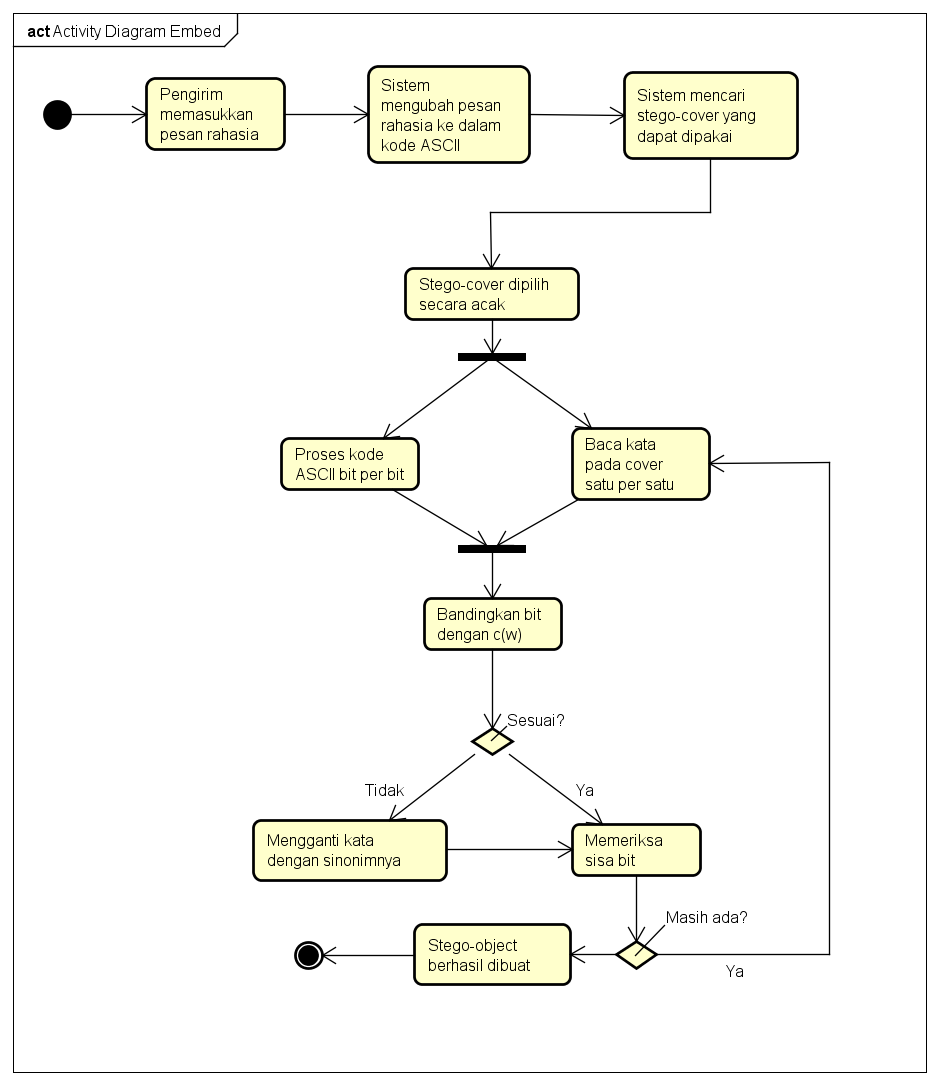
\includegraphics[scale=0.4]{Gambar/activity-penyisipan}
	\caption{Activity Diagram perangkat lunak steganografi saat menyisipkan} 
	\label{fig:4_activity-penyisipan}
\end{figure}

Diagram aktivitas ekstraksi dapat dilihat pada Gambar \ref{fig:4_activity-ekstraksi}

\begin{figure}[H]
	\centering
	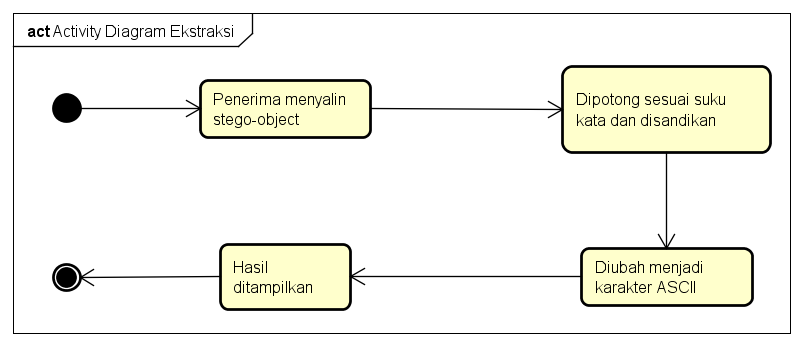
\includegraphics[scale=0.5]{Gambar/activity-ekstraksi}
	\caption{Activity Diagram perangkat lunak steganografi saat proses ekstraksi} 
	\label{fig:4_activity-ekstraksi}
\end{figure}

Dari diagram aktivitas di atas dapat dijelaskan sebagai berikut:

\begin{enumerate}
	\item Penerima akan memberikan input berupa \textit{stego-object} dari program yang sama.
	\item Sistem lalu akan memenggal kata-kata yang ada untuk mendapatkan banyak suku katanya. Setelah itu dilakukan penyandian, angka 0 untuk kata dengan banyak suku kata genap dan angka 1 untuk jumlah ganjil.
	\item Selesai melakukan penyandian, hasilnya akan diubah menjadi karakter ASCII yang sesuai.
	\item Kini sudah didapatkan pesan dengan karakter ASCII, hasil akan ditampilkan pada layar.
\end{enumerate}